\chapter{Experiments}
\label{chap:experiments}
In this section, we describe the experiments we conducted.
We start with the human evaluation, then move onto \ac{ml} models.
To assess the performance of a keywords-based model we trained 
a \ac{mlr}.  A possible high performance of
this model would mean that the tasks are solvable only by spotting typical keywords
for the classes without any deeper understanding. Subsequently,
we fine-tune Czech pre-trained Transformers on our tasks to evaluate
the importance of textual dependencies for the tasks. Lastly, we fine-tune
GPT-3 to evaluate its multi-lingual capabilities and compare the model to the
substantially smaller Czech Transformers.

\section{Human Performance}
\label{sec:human}
To evaluate human performance, we let four evaluators classify the articles on 
the Test Human set (\autoref{sec:splits}).
Each evaluator got access to Google Sheet\footnote{https://docs.google.com/},
where they had to assign each document a correct label for each task.
Evaluators were offered all options for each task, not just the subset from the Test Human set.
We will denote averaged scores of all evaluators as \textbf{Human}.

\section{Baseline Model}
\label{sec:baseline-exp}
We used \ac{mlr} with TF-IDF features.
Following \textcite{strakaSumeCzechLargeCzech2018a}, we included the following features:
\begin{itemize}
    \item Number of words
    \item Number of words with only non-alphabetic characters
    \item Number of uppercase words
    \item Number of digits words
    \item Number of capitalized words
\end{itemize}
We  used 1-2 grams with a maximum document frequency of 1\% and MosesTokenizer\footnote{\url{https://pypi.org/project/mosestokenizer/}}
with Czech stop words\footnote{\url{https://pypi.org/project/stop-words/}} on lowercase text as a tokenization method.
We then run a grid search over Inverse Regularization term with values $1, 10, 100, 1000$
and selected the model with the highest F1 Macro score on the validation set.
As for the solver, we used SAGA~\parencite{defazioSAGAFastIncremental2014}
implementation from Scikit-learn library\footnote{\url{https://scikit-learn.org}},
with max iterations set to 800 and an early stopping tolerance of 0.001.

With this setting, we created 2 models; \textbf{LR-50} with 50k TF-IDF features
and \textbf{LR-200} with 200k TF-IDF features.

\section{Pre-trained Transformers}
\label{sec:backbone}
For backbone models, we employed \textbf{RobeCzech}, \textbf{Fernet-News},
and \textbf{GPT-3}. We chose RobeCzech and Fernet-News as both are Czech mono-lingual transformers
with the same architecture and the relatively same number of parameters~(\autoref{tab:czech-monolingual}).
The main difference is the training data and training setting~(\autoref{sec:robe-czech}, \autoref{sec:fernet}).
We hypothesized
that the similarity of task and Fernet-News domains would lead to better task
performance.

\subsection{RobeCzech and Fernet-News}
\label{sec:base-models}

\begin{figure}[h]
    \centering
    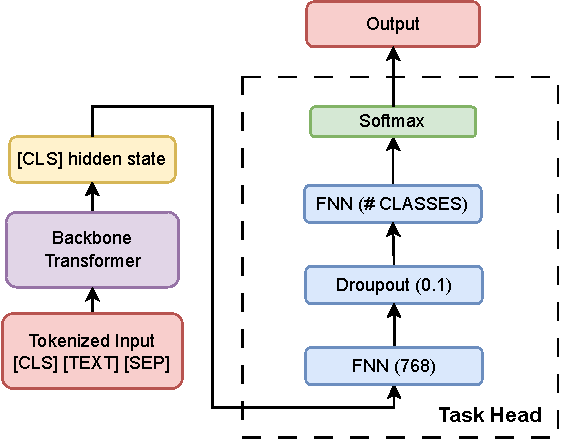
\includegraphics[width=0.7\linewidth]{img/transformer/fine_tune.pdf}
    \caption{Fine-tuning architecture for the classification task.}
    \label{fig:class-tune}
\end{figure}

For fine-tuning, we mostly followed hyperparameter settings
recommend by \textcite{sunHowFineTuneBERT2020}.
As for architecture, we took the backbone model and replaced
the head as shown in~\autoref{fig:class-tune}.
We fine-tuned both models for 2 epochs with linear decay, 0.1 warmup, 48
effective batch size, and AdamW as the optimizer. All layers were unfrozen
except for the embedding layer. Learning rates were selected based on the best
validation score of a grid search over a 0.4 fraction of the training data. Possible
learning rate values were:
\begin{enumerate}
    \item RobeCzech: 3e-5, 4.5e-5, 7.5e-5
    \item Fernet-News: 1e-5, 2e-5, 3e-5
\end{enumerate}
The proposed learning rate values for RobeCzech and Fernet-News differ due
to the divergence of Fernet-News with higher learning rates. To deal with long
texts, we chose to truncate them to the first 510 tokens

For implementation, we used \textit{Pytorch Lightning 2.0}\footnote{\url{https://www.pytorchlightning.ai/}},
\textit{\ac{hf} Transformers 4.24}\footnote{\url{https://huggingface.co/docs/transformers/index}}
and \textit{Pytorch 2.0.0}\footnote{\url{https://pytorch.org/}}.
We trained models on \ac{aic} with a single GeForce RTX 2080 Ti.
We denote the models as \textbf{R-Base} and \textbf{F-Base}.

\subsection{GPT-3}
\label{sec:gpt-3}
We chose the Ada version of GPT-3, as it is the cheapest.
Ada costs 0.00004\$/1k tokens for fine-tuning and 0.00016\$/1k tokens for inference.
The model was trained in a multi-task setting, utilizing the article text
(query) and corresponding task labels in Czech (text completion) as input. For
example, a sample text completion might be:
\begin{quote}
    "Deník.cz Sport Žena Pondělí"
\end{quote}

The Ada model takes a maximum of 2048 tokens; thus, we truncated documents to the first 1400 characters.
To save the costs, we used \textbf{Train-small} for fine-tuning and
\textbf{Test-small} (see \autoref{sec:splits}) for inference.
We finetuned for 2 epochs.

For comparison, we fine-tuned and evaluated RobeCzech and Fernet-News on the same splits.
We denote the models as \textbf{GPT-3}, \textbf{R-Small} and \textbf{F-Small}.

\section{Fine-tuning Enhancements}
\label{sec:finetuning}
We were interested in ways to improve fine-tuning performance without changing the backbone model.
We tested three approaches inspired by \textcite{howardUniversalLanguageModel2018a} and \textcite{sunHowFineTuneBERT2020}.
All the experiments were done on \textbf{RobeCzech} model, with settings as in \autoref{sec:base-models}
unless stated otherwise.

\subsection{Truncation}
\label{sec:truncation}
The base models are trained with truncation to the first 510 tokens.
Due to the nature of the task,
we hypothesized that the last part of the article might contain more relevant information:
\begin{quote}
    Pro Idnes.cz Jana Křížová
\end{quote}
Therefore, we truncated the text by taking the last 510 tokens.
We denote the model as \textbf{Truncate}.

\subsection{\acl{flm}}
\label{sec:task-modeling}
Both \textcite{howardUniversalLanguageModel2018a} and \textcite{sunHowFineTuneBERT2020}
found that \acf{flm} on task dataset can improve performance.
We thus further pre-trained RobeCzech on the content of the article in FULL-SENTENCES setting~\parencite{liuRoBERTaRobustlyOptimized2019}
with a batch size of 192 and a learning rate of 5e-5 for
10 epochs.  We then used the pre-trained model as the backbone and trained with the same setting as the Base model.
We denote the resulting model as \textbf{LM-Tune}.

\subsection{Gradual Unfreezing with Discriminative Learning Rates}
\label{sec:gradual-unfreezing}
\textcite{howardUniversalLanguageModel2018a} showed that we could improve model performance by gradually unfreezing layers.
As the original method was used on RNNs, we were interested if it would work with Transformers.
We also added a discriminative learning rate which sets a smaller learning rate for the lower layers.
We set the discriminative factor to 0.95 as in \parencite{sunHowFineTuneBERT2020}.
The \ac{gu} is not well described in \parencite{howardUniversalLanguageModel2018a}, thus we tried two approaches:
\begin{enumerate}
    \item \textbf{Grad-12} Unfreeze 1 layer per epoch, starting from the last layer, and run for 12 epochs.
    \item \textbf{Grad-24} Unfreeze 1 layer per epoch,
    starting from the last layer, and run for 24 epochs~(12 epochs in the full unfrozen state).
\end{enumerate}
The epoch lengths were adjusted, so that the total number of optimizer steps stays the same as in \autoref{sec:base-models}~(full 2 epochs).
For both approaches, we unfroze the classifier layer at the start of training with the learning rate decaying from 1e-3 to 5e-5.
The remaining layers were adjusted based on the discriminative learning rate.
Each unfrozen layer had a scheduler with the same setting as Base models~(\autoref{sec:backbone}).
However, it started scheduling when the layer was unfrozen.

\section{Final Model}
\label{sec:final-model}
Finally, we created a model combining the best pre-trained transformer and fine-tuning approaches.
Therefore, we used \textbf{RobeCzech} as a backbone with \ac{flm}.
Additionally, we reused the classifier scheduling as in \autoref{sec:gradual-unfreezing}.
Due to the great results on the restricted dataset, we also lowered the warmup steps to just 0.01 and added
Most-recent sampling.
\subsection{Most-recent Sampling}
To add weight to more recent articles, we sampled article $i$ from the dataset with the following probability:
\begin{equation*}
    P(i) = \frac{\exp(2 d_i)}{\sum_{j=1}^{n} \exp(2 d_j)}
\end{equation*}
where $d_i$ equals:
\begin{equation*}
    d_i = \frac{t_i}{\max_{0\le j \le n}{t_j}}
\end{equation*}
and where $t_i$ is the time difference between the published date of article $i$ and the dataset's eldest article in days.
